\documentclass[19pt]{extarticle}
\usepackage{fontspec}
\setmainfont{LiberationSans}[
  Path=fonts/,
  Extension=.ttf,
  UprightFont=*-Regular,
  BoldFont=*-Bold,
  ItalicFont=*-Italic,
  BoldItalicFont=*-BoldItalic
]
\usepackage[paperwidth=594mm,paperheight=841mm,margin=10mm]{geometry}
\pagestyle{empty}
\setlength{\parindent}{0pt}
\usepackage{xcolor}
\usepackage{tcolorbox}
\tcbuselibrary{skins}
\usepackage{graphicx}
\usepackage{booktabs}
\usepackage{array}
\usepackage{enumitem}
\usepackage{tikz}

\definecolor{teal}{HTML}{14505C}
\definecolor{bars}{HTML}{E8B183}
\definecolor{rule}{HTML}{D9B49A}
\definecolor{ink}{HTML}{1B3A3F}

\setlist[itemize]{leftmargin=1.1em,itemsep=0.15em,topsep=0.2em,parsep=0pt}

\newcommand{\sectionbar}[1]{%
  \colorbox{bars}{\makebox[\dimexpr\linewidth-2\fboxsep][l]{\strut\bfseries\color{ink}\fontsize{26}{30}\selectfont #1}}%
}

\newtcolorbox{block}[1]{%
  enhanced, colback=white, colframe=rule, boxrule=0.5pt,
  arc=1mm, left=2.5mm, right=2.5mm, top=1.5mm, bottom=2mm,
  before skip=6.5mm, after skip=0pt,
  fonttitle=\bfseries,
  title={}, coltitle=ink,
}

\begin{document}

% ---------------------------------------------------------------- header
\begin{tikzpicture}[remember picture, overlay]
  \node[anchor=north west] at ([xshift=10mm,yshift=-8mm]current page.north west)
    {\setlength{\fboxsep}{4mm}\fbox{\parbox[c][12mm][c]{26mm}{\centering\Large\bfseries\color{ink}80}}};
\end{tikzpicture}

\vspace*{2mm}
\begin{center}
  {\fontsize{46}{52}\selectfont\bfseries\color{teal}
   Typed Judgment, Deterministic Enforcement:\\[1mm]
   A Consent-Gated Gateway Architecture for Inter-Agent Collaboration over Messaging Channels}

  \vspace{5mm}
  {\Large\color{ink}\bfseries
   Yizhang Cai\textsuperscript{1}\quad Jun Liu\textsuperscript{1}\quad
   Di Ma\textsuperscript{2}\quad Ke Yu\textsuperscript{1}\quad Ke Li\textsuperscript{1}}

  \vspace{3mm}
  \begin{tcolorbox}[enhanced, sharp corners, colback=white, colframe=teal,
    boxrule=0.4pt, width=\textwidth, halign=center,
    borderline={0.4pt}{0pt}{teal,dashed}, fontupper=\normalsize]
    \textsuperscript{1}School of Artificial Intelligence, Beijing University of Posts and
    Telecommunications\quad\textsuperscript{2}Beijing Guoshu Zhilian Technology Co., Ltd.\\
    \texttt{2025111259@bupt.cn}\quad\textbar\quad Special Session XII: Agent Interconnection and
    Collaboration Intelligence
  \end{tcolorbox}
\end{center}

\vspace{2mm}

% ---------------------------------------------------------------- body
\begin{minipage}[t]{0.482\textwidth}
\vspace{0pt}
\begin{block}{}
\sectionbar{Introduction}
\vspace{2mm}

Messaging channels deliver human events that are unstructured, duplicated,
delayed, or replayed, while agent protocols expect authenticated endpoints,
structured requests, and explicit task state. A gateway therefore has to decide
whether a message requests work, which agent is eligible, whether consent is
needed, and whether an event is a replay or an injection.

We separate bounded model judgment from deterministic enforcement: the model
answers closed questions, and policy code owns thresholds and every effect.
\end{block}

\begin{block}{}
\sectionbar{Objectives}
\vspace{2mm}

\begin{itemize}
  \item Seven modules from an iMessage/Photon ingress to an ACPs/AIP v2.2
        Leader--Partner path.
  \item Four invariants kept in code: authorization, identity, isolation,
        idempotency.
  \item A judgment plane of seven closed questions (J1--J7) that can only
        parameterize thresholds.
  \item Live measurement of routing, consent, and the deployed advisory path.
\end{itemize}
\end{block}

\begin{block}{}
\sectionbar{Judgment plane}
\vspace{2mm}
The layer returns closed labels or probabilities only: it cannot emit free text
or call a tool, and it only parameterizes policy thresholds.

\vspace{2mm}
\begin{tabular}{@{}ll@{}}
\textbf{J1} intent & \textbf{J2} routing \\
\textbf{J3} ambiguity & \textbf{J4} consent \\
\textbf{J5} replay & \textbf{J6} retryability \\
\textbf{J7} injection & \\
\end{tabular}
\end{block}

\begin{block}{}
\sectionbar{Materials and Methods}
\vspace{2mm}

\begin{itemize}
  \item M1 ingress authentication; M2 caller/conversation isolation;
        M3 discovery and routing; M4 consent; M5 identity-bound execution;
        M6 state, idempotency and recovery; M7 delivery and telemetry.
  \item 130 generated requests through the real ingress, three deliveries each;
        paired same-code ablations on staging copies; consent trials on the
        deployed adapter; a 280-item judgment suite sampled three times.
\end{itemize}

\vspace{2mm}
\centering
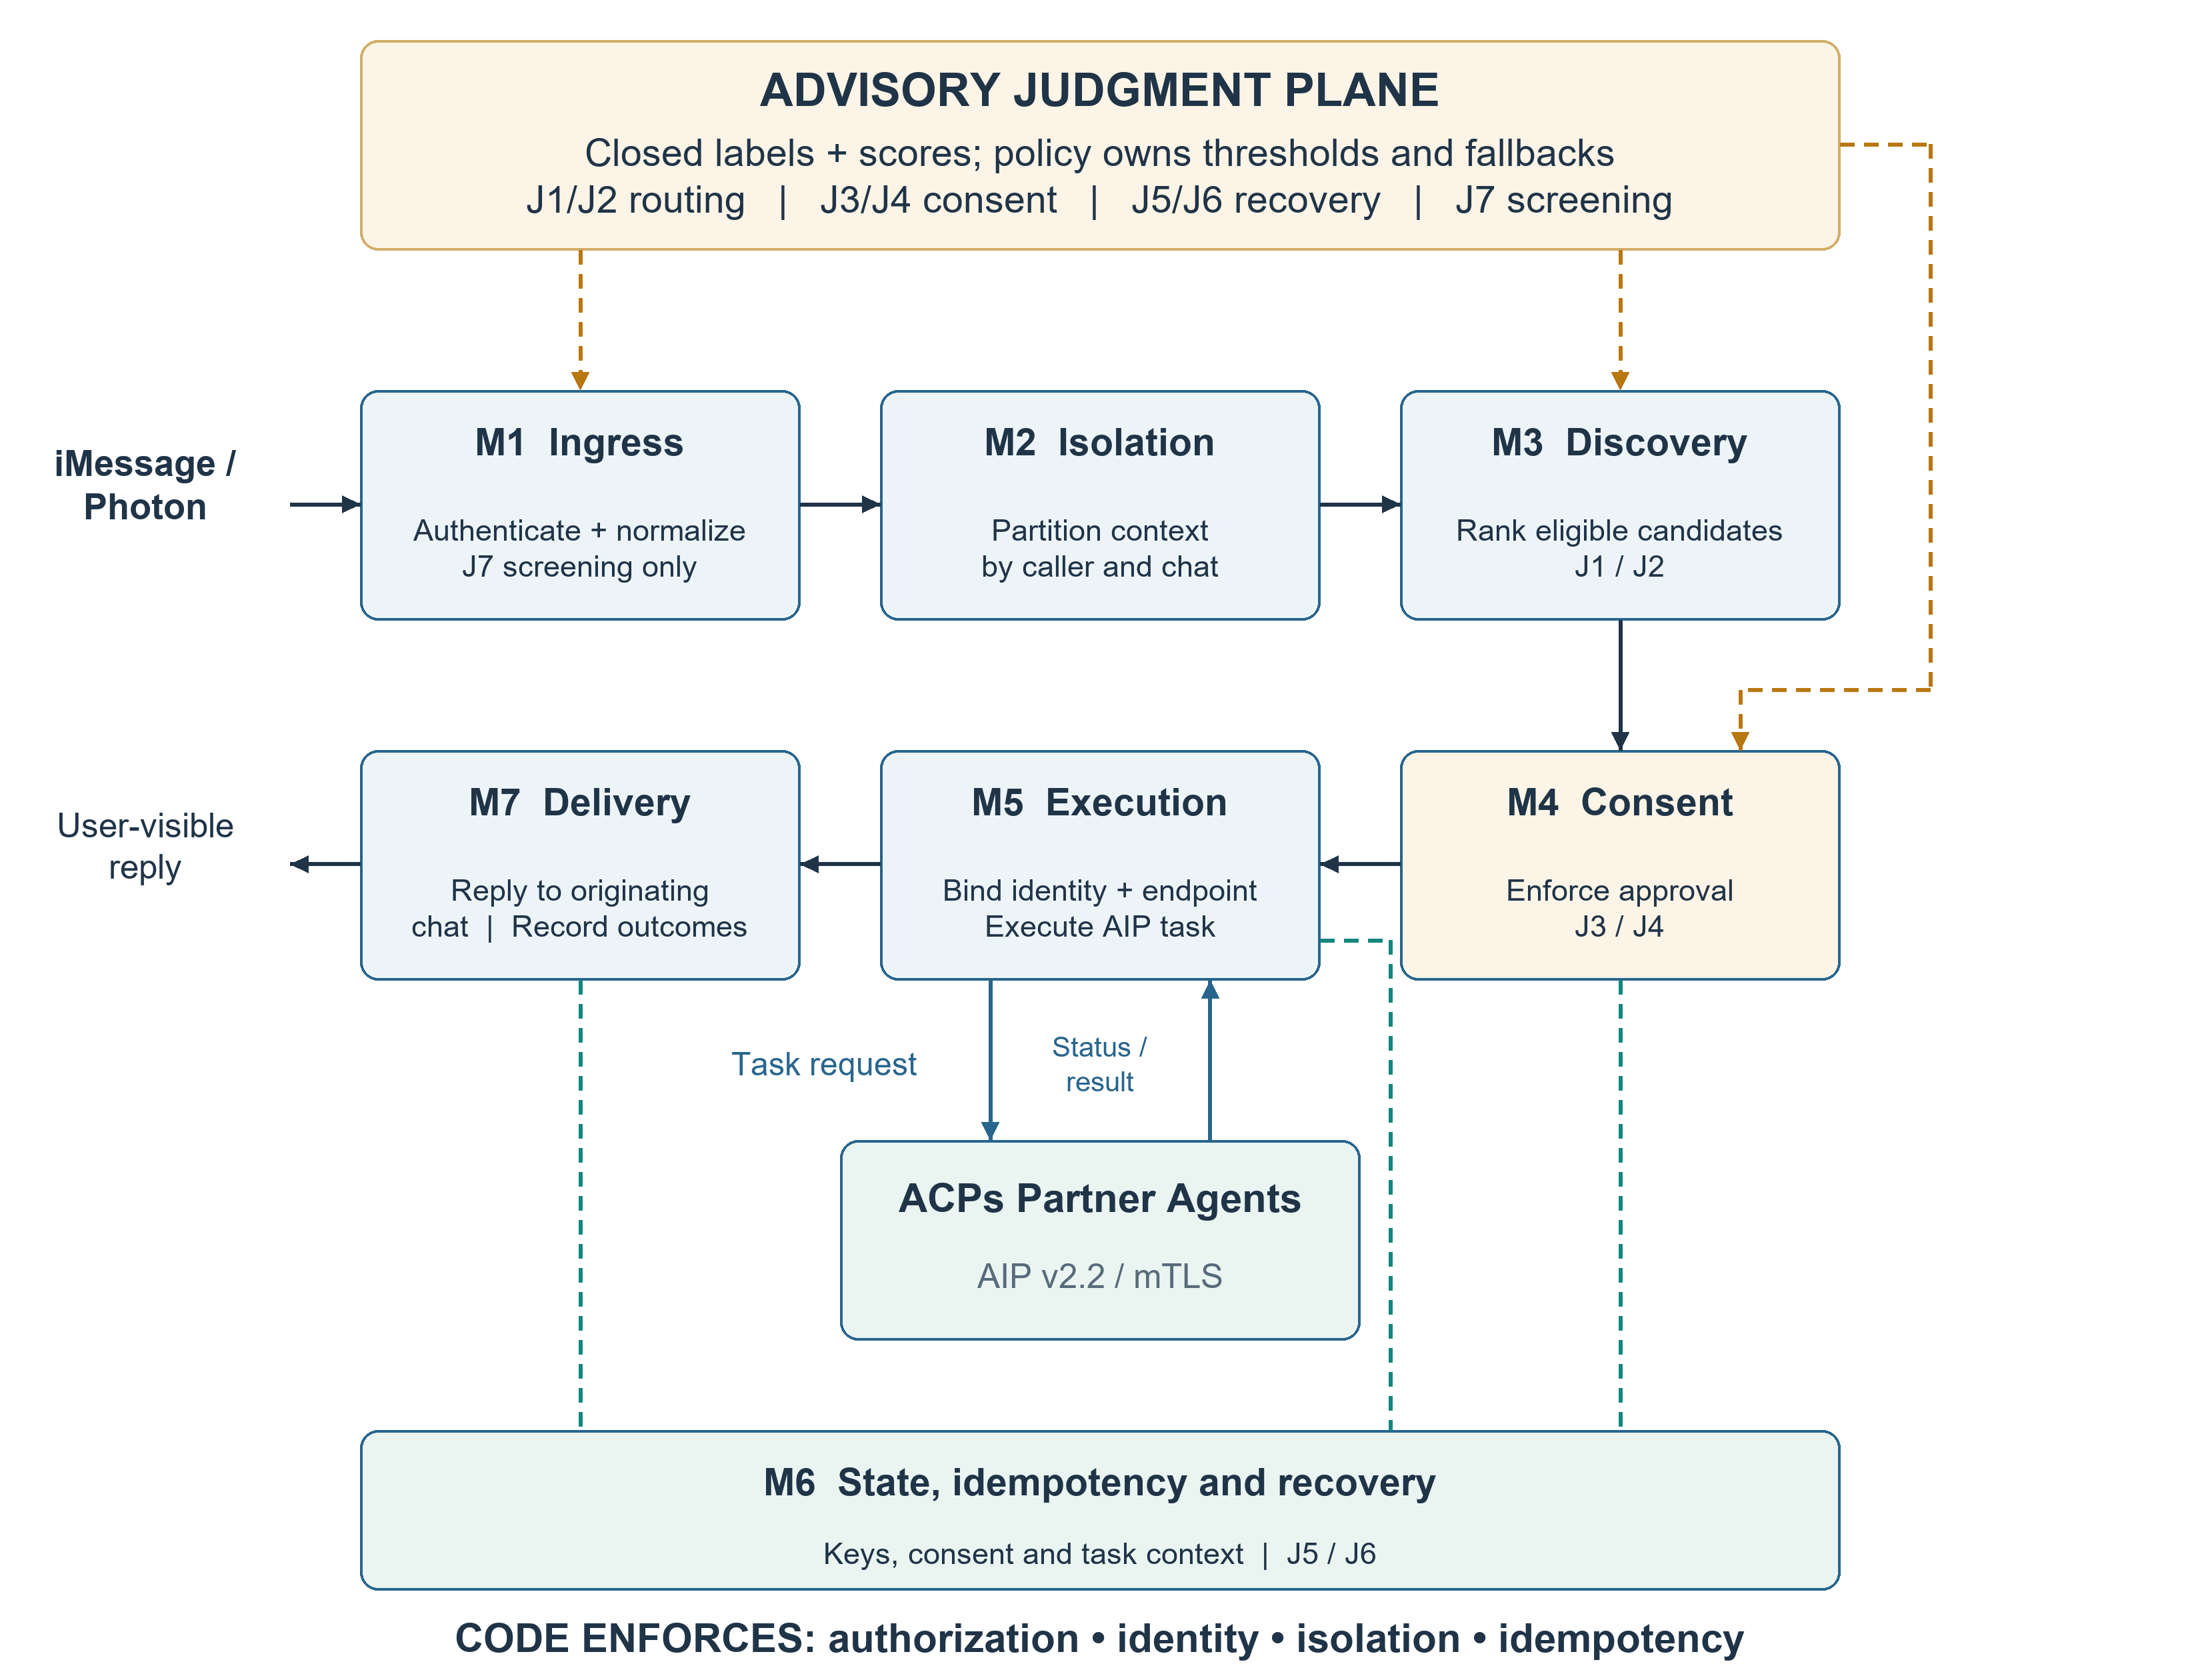
\includegraphics[width=1.0\linewidth]{../figures/fig1_architecture.png}

\vspace{1mm}
\raggedright
\small\textbf{Figure 1.} Seven modules, four invariants, and the advisory
judgment plane.
\end{block}

\begin{block}{}
\sectionbar{Contributions}
\vspace{2mm}
\begin{itemize}
  \item A seven-module gateway that separates bounded judgment from
        deterministic enforcement in code.
  \item Four invariants enforced by the runtime rather than by prompts.
  \item A judgment plane of seven closed questions that cannot act on its own.
  \item A live evaluation of routing, consent and advisory judgment, with a
        released artifact.
\end{itemize}
\end{block}

\begin{block}{}
\sectionbar{Evaluation setup}
\vspace{2mm}
\small
\begin{tabular}{@{}l@{\hspace{6mm}}l@{}}
Requests & 130 generated, 3 deliveries each \\
Consent & 30 trials + 10 redeliveries \\
Judgment suite & 280 items, 3 runs \\
Injection stress & 200 injected, 256 benign \\
\end{tabular}
\end{block}

\begin{block}{}
\sectionbar{At a glance}
\vspace{2mm}
\centering
\begin{minipage}{0.46\linewidth}
\centering
{\fontsize{26}{30}\selectfont\bfseries\color{teal}48/48/50}\\[0.5mm]
{\small target recommended (of 50)}
\end{minipage}\hfill
\begin{minipage}{0.46\linewidth}
\centering
{\fontsize{26}{30}\selectfont\bfseries\color{teal}0/30 $\rightarrow$ 30/30}\\[0.5mm]
{\small identity ablation}
\end{minipage}

\vspace{3mm}
\begin{minipage}{0.46\linewidth}
\centering
{\fontsize{26}{30}\selectfont\bfseries\color{teal}36/36}\\[0.5mm]
{\small one action per consent}
\end{minipage}\hfill
\begin{minipage}{0.46\linewidth}
\centering
{\fontsize{26}{30}\selectfont\bfseries\color{teal}94.1\% vs 83.9\%}\\[0.5mm]
{\small typed vs free text}
\end{minipage}
\end{block}

\end{minipage}\hfill
\begin{minipage}[t]{0.482\textwidth}
\vspace{0pt}
\begin{block}{}
\sectionbar{Results}
\vspace{2mm}

\textbf{Routing.} The generated target was recommended for 48/48/50 of 50
direct requests; 39/38/38 of 40 ambiguous requests received more than one agent;
0/40 out-of-scope requests recommended a study partner.

\vspace{1.5mm}
\centering
\begin{tabular}{@{}lcc@{}}
\toprule
\textbf{Ablation} & \textbf{Control} & \textbf{Removed} \\
\midrule
Identity binding & 0/30 & 30/30 \\
Caller isolation & 0/30 & 30/30 \\
Idempotency & 30 exec. & 60 exec. \\
\bottomrule
\end{tabular}
\vspace{1.5mm}
\raggedright

\textbf{Consent.} No partner action before consent (0/40); every consent
produced exactly one action (36/36).

\vspace{1.5mm}
\centering
\begin{tabular}{@{}lcc@{}}
\toprule
 & \textbf{Typed} & \textbf{Free text} \\
\midrule
Accuracy & 94.1\% & 83.9\% \\
Brier & 0.095 & 0.266 \\
ECE & 0.026 & 0.144 \\
\bottomrule
\end{tabular}
\vspace{1mm}
\raggedright
\small 280 items, three runs, human-verified labels. The injection stress set
(200 injected, 256 benign) misses none but flags about half of quoted mentions,
which is why the injection score only parameterizes policy.

\vspace{2mm}
\centering
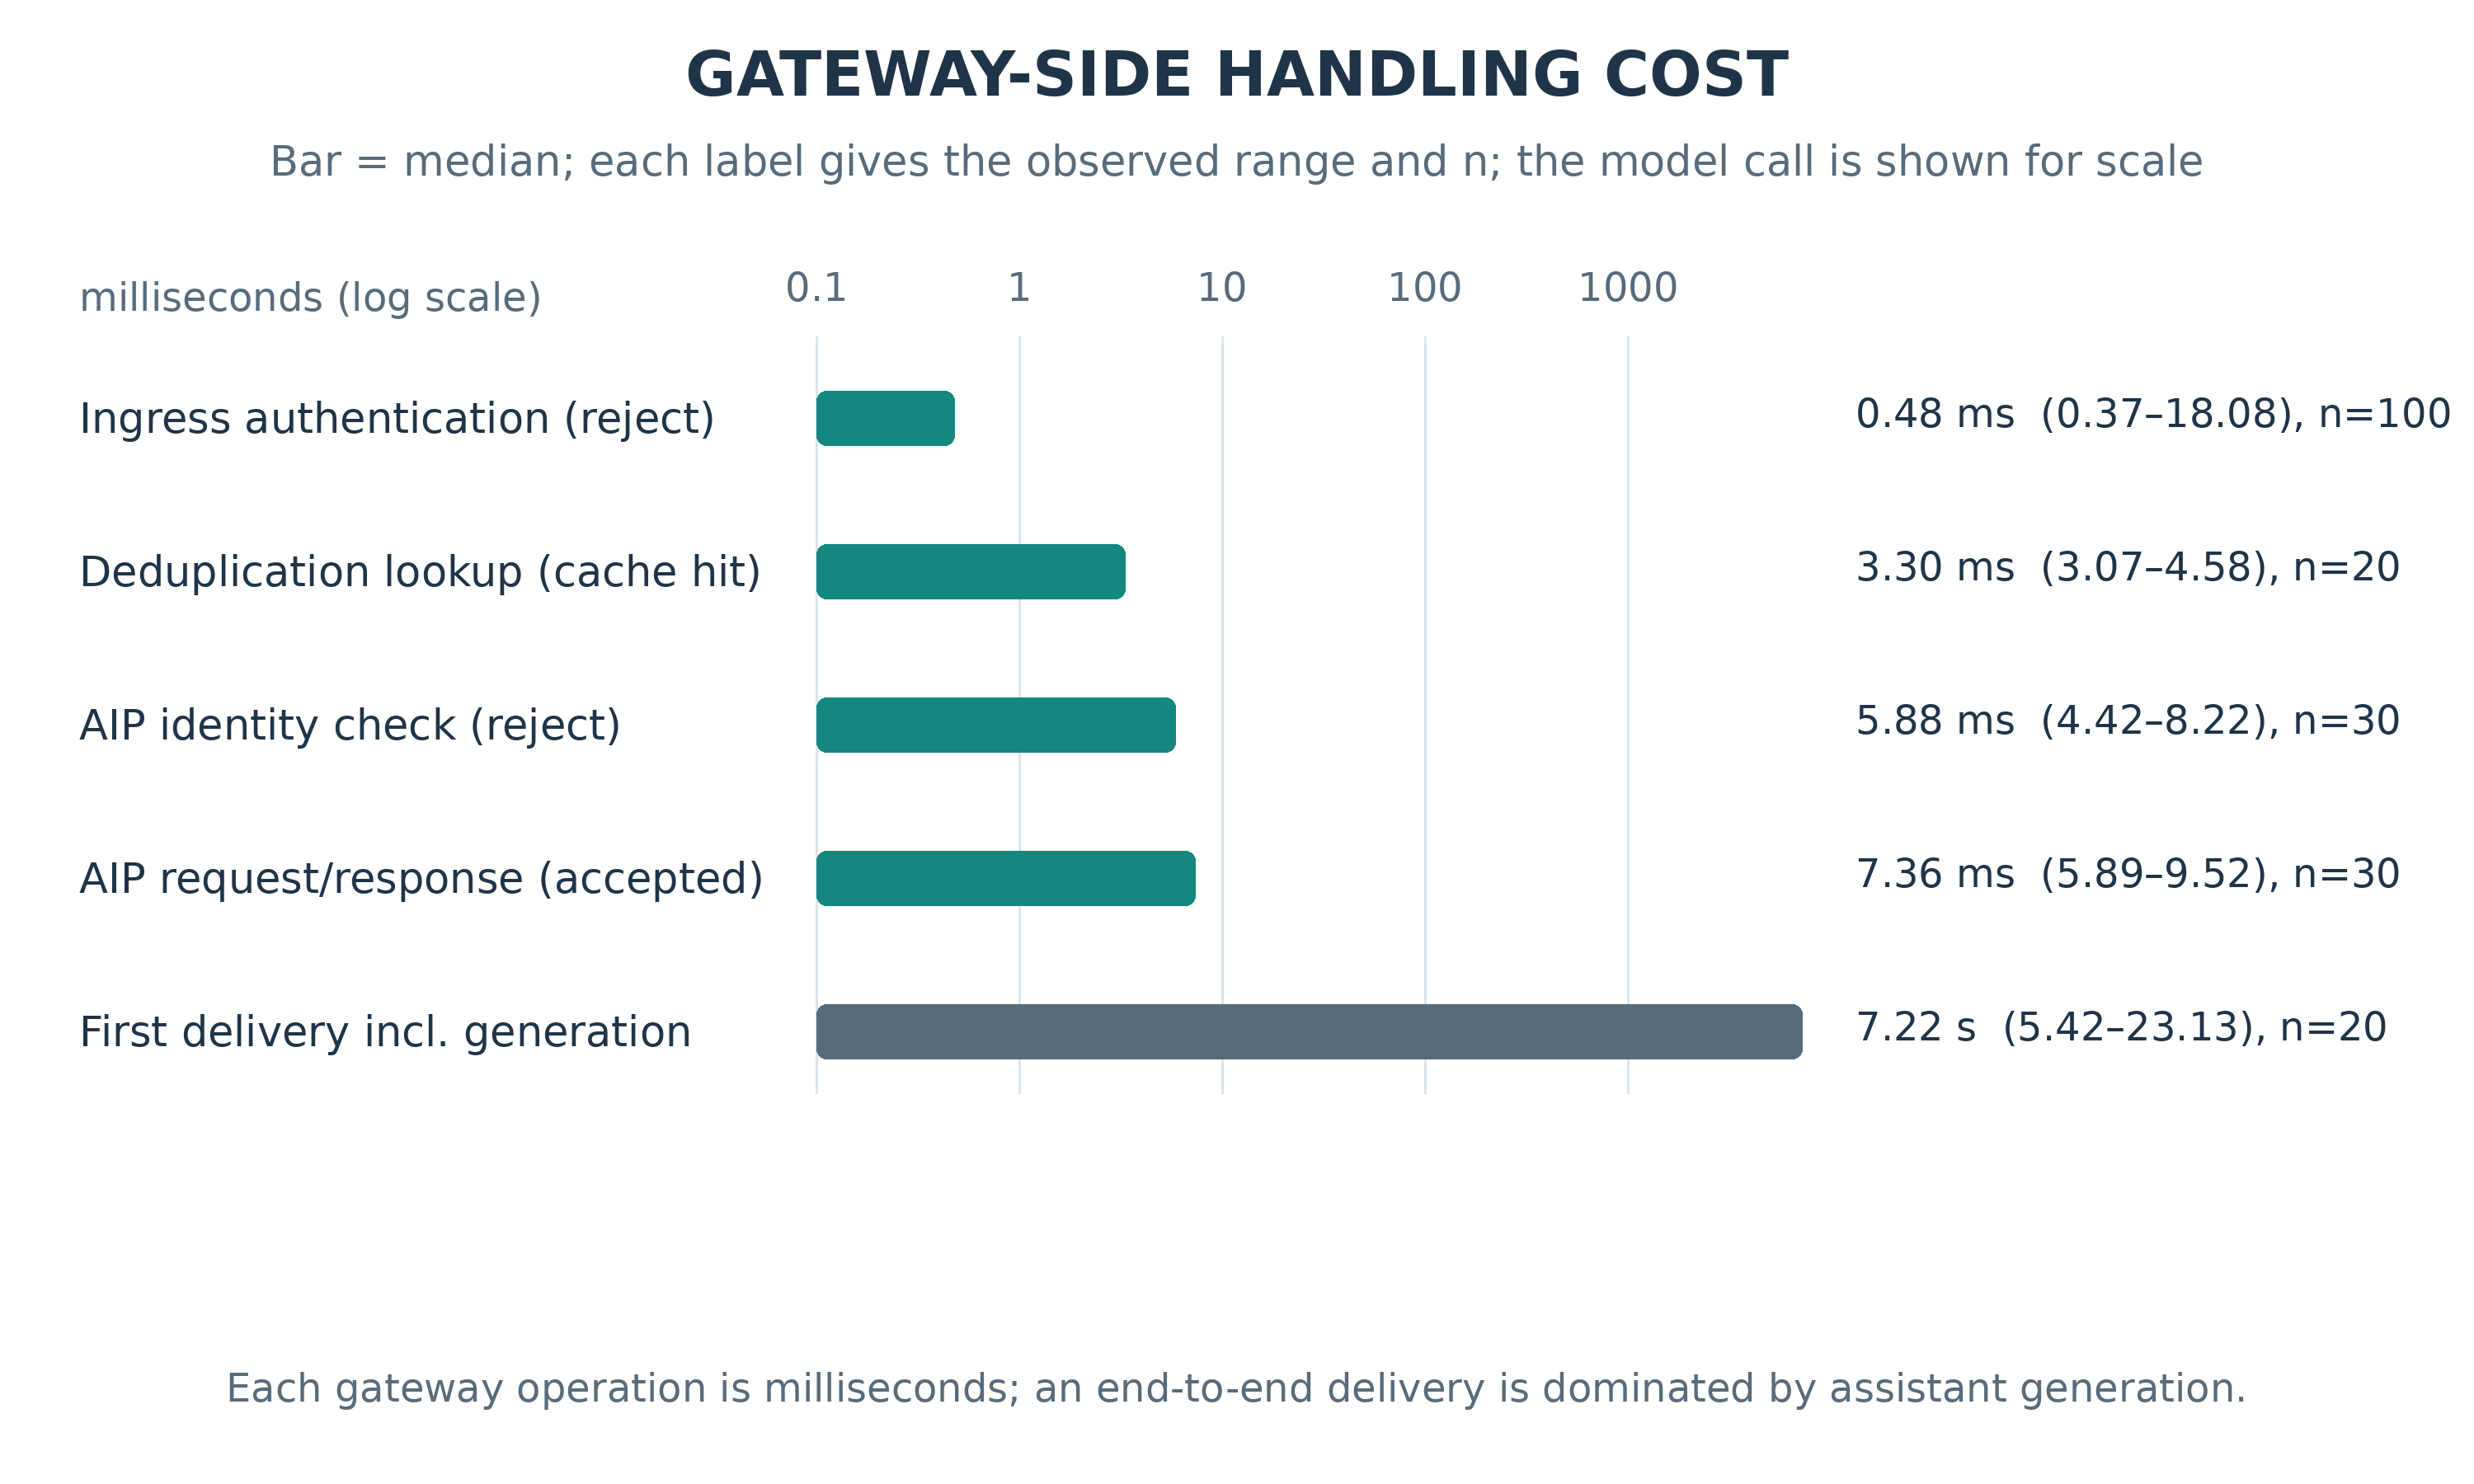
\includegraphics[width=0.88\linewidth]{../figures/fig3_overhead.png}

\vspace{1mm}
\raggedright
\small\textbf{Figure 3.} Median gateway-side handling cost per operation.
\end{block}

\begin{block}{}
\sectionbar{Processing flow}
\vspace{2mm}
\centering
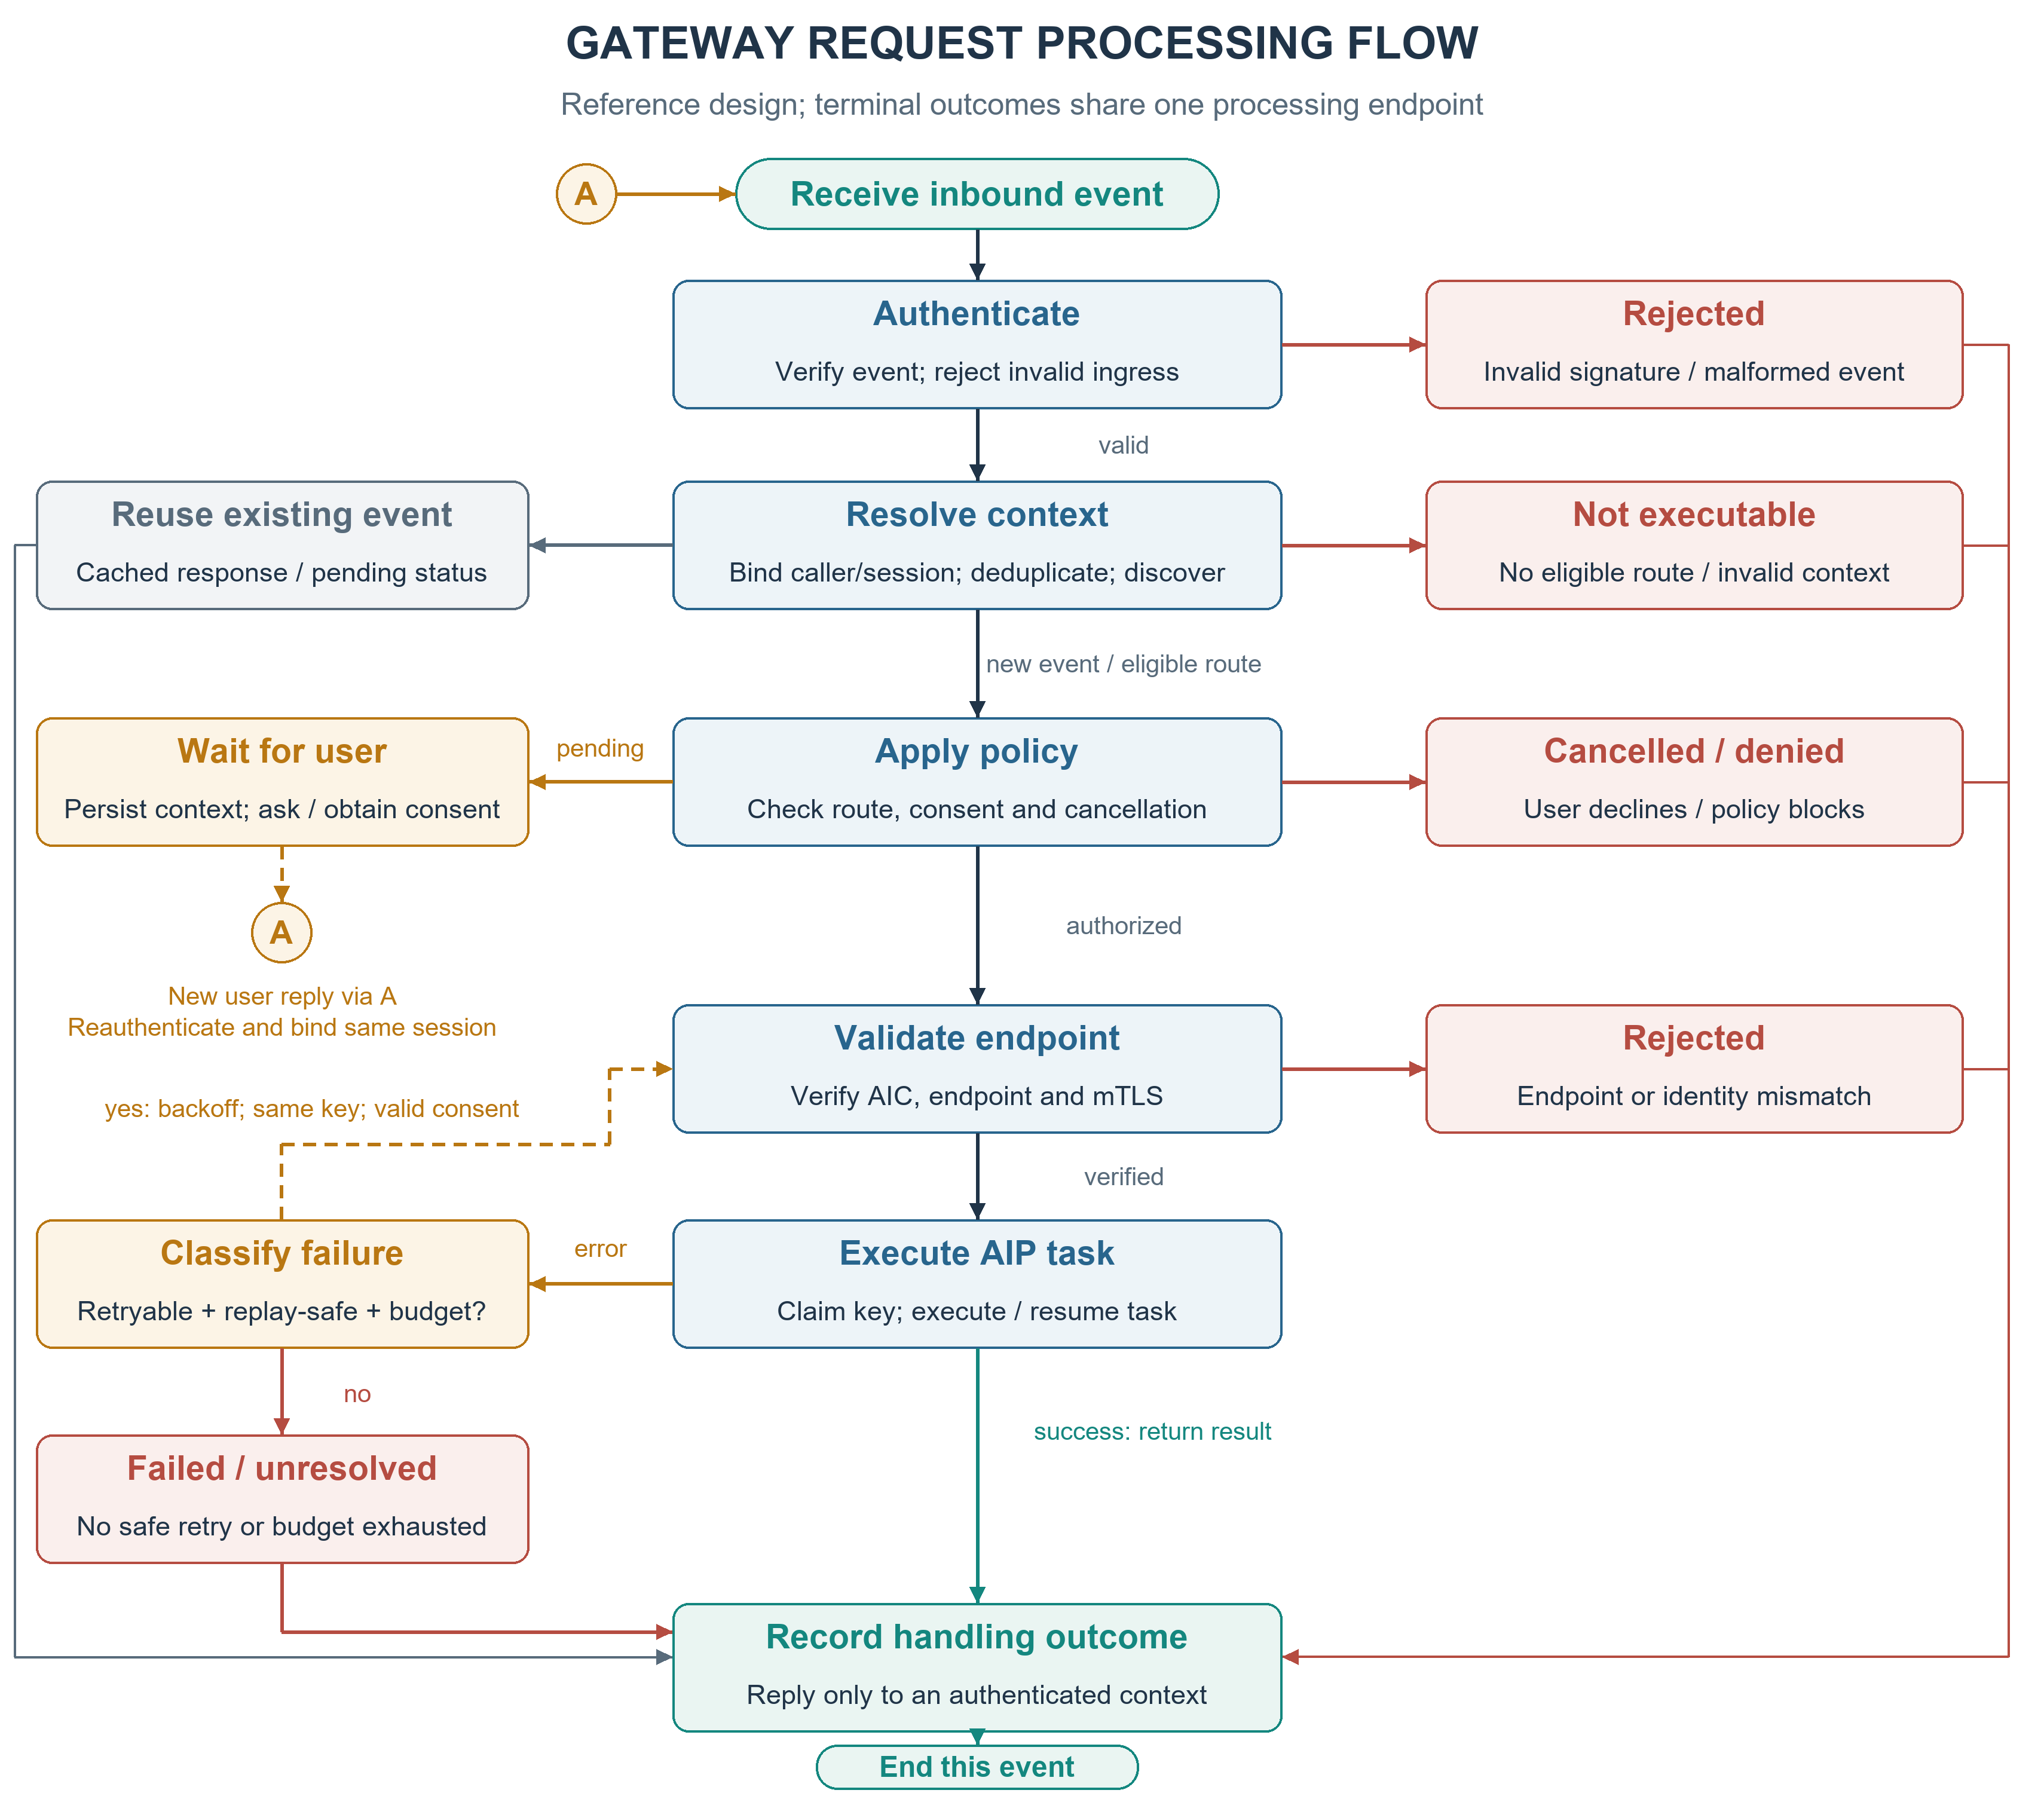
\includegraphics[width=0.86\linewidth]{../figures/fig2_state_machine.png}

\vspace{1mm}
\raggedright
\small\textbf{Figure 2.} Deduplication precedes every model call; a pending
consent re-enters at authentication; a failed identity or endpoint check never
reaches execution.
\end{block}

\begin{block}{}
\sectionbar{Conclusion}
\vspace{2mm}

The model advises; code controls identity, state, and every side effect. Typed
answers are more accurate and better calibrated than free text, and consent
gating admits exactly one partner action per accepted event.
\end{block}

\begin{block}{}
\sectionbar{References}
\vspace{1.5mm}
{\small
\mbox{[1]} J. Liu et al., ACPs: Agent Collaboration Protocols for the Internet of Agents, arXiv:2505.13523, 2025.\par
\mbox{[2]} Q. Zhan et al., InjecAgent, arXiv:2403.02691, 2024.\par
\mbox{[3]} S. Chen et al., StruQ, arXiv:2402.06363, 2024.\par
\mbox{[4]} E. Debenedetti et al., AgentDojo, NeurIPS 2024.}
\end{block}

\begin{block}{}
\sectionbar{Contact}
\vspace{1.5mm}
{\small
Paper 80\quad\textbar\quad JCRAI 2026, Special Session XII\\
Yizhang Cai, \texttt{2025111259@bupt.cn}\\
Artifact: \texttt{github.com/ankelas/consent-gated-gateway-artifact}\\
Supported by S\&T Program of Xiongan New Area (No. XA2026111001K).}
\end{block}

\end{minipage}

\vspace{4mm}


\begin{tikzpicture}
  \draw[rule, line width=0.4pt] (0,0) -- (\dimexpr\textwidth-0.5pt\relax,0);
  \node[anchor=north] at (0.5\textwidth,-2mm)
    {\small\color{ink}2026 6th International Joint Conference on Robotics and
     Artificial Intelligence (JCRAI 2026)\quad\textbar\quad SS12\quad\textbar\quad Paper 80};
\end{tikzpicture}

\end{document}
